% !TeX program = xelatex
%%%%%%%%%%%%%%%%%%%%%%%%%%%%%%%%%%%%%%%%%%%%%%%%%%%%%%%%%%%%%%%%%%%%%%%%
% Plantilla Póster TFG/TFM
% Escuela Politécnica Superior de la Universidad de Alicante
% Realizado por: Jose Manuel Requena Plens
% Contacto: info@jmrplens.com / Telegram:@jmrplens
%%%%%%%%%%%%%%%%%%%%%%%%%%%%%%%%%%%%%%%%%%%%%%%%%%%%%%%%%%%%%%%%%%%%%%%%

%%%%%%%%%%%%%%%%%%%%%%%%%%%%%%%%%%%%%%%%%%%%%%%%%%%%%%%%%%%%%%%%%%%%%%
% INDICA TU TITULACIÓN
% ID	GRADO -------------------------------------------------
% 1		Ingeniería en Imagen y Sonido en Telecomunicación
% 2		Ingeniería Civil
% 3		Ingeniería Química
% 4		Ingeniería Informática
% 5		Ingeniería Multimedia
% 6		Arquitectura Técnica
% 7		Arquitectura
% 8		Robótica
% %		%%%%%%%%%%%%
% ID	MÁSTER ------------------------------------------------
% A		Telecomunicación
% B		Caminos, Canales y Puertos
% C		Gestión en la Edificación
% D		Desarrollo Web
% E		Materiales, Agua, Terreno
% F		Informática
% G 	Automática y Robótica
% H		Prevención de riesgos laborales
% I		Gestión Sostenible Agua
% J		Desarrollo Aplicaciones Móviles
% K		Ingeniería Química
% L		Ciberseguridad
%%%%%%%%%%%%%%%%%%%%%%%%%%%%%%%%%%%%%%%%%%%%%%%%%%%%%%%%%%%%%%%%%%%%%%%%%
%!!!!!!!!!!!!!!!!!!!!!!!!!!!!!!!!!!!!!!!!!!!!!!!!!!!!!!!!!!!!!!!!!!!!!%%%
																		%
\def\IDtitulo{1} % INTRODUCE LA ID DE TU TITULACIÓN						%
																		%
%!!!!!!!!!!!!!!!!!!!!!!!!!!!!!!!!!!!!!!!!!!!!!!!!!!!!!!!!!!!!!!!!!!!!!%%%
%%%%%%%%%%%%%%%%%%%%%%%%%%%%%%%%%%%%%%%%%%%%%%%%%%%%%%%%%%%%%%%%%%%%%%%%%

%%%%%%%%%%%%%%%%%%%%%%%%%%%%%%%%%%%%%%%%%%%%%%%%%%%%%%%%%%%%%%%%%%%%%%
% INFORMACIÓN DEL TFG
%%%%%%%%%%%%%%%%%%%%%%%%%%%%%%%%%%%%%%%%%%%%%%%%%%%%%%%%%%%%%%%%%%%%%%
\def\titulo{Título del Trabajo de Fin de Grado/Máster}
\def\autor{Nombre y Apellidos}

% Archivo .TEX que incluye todas las configuraciones del documento y los paquetes. Añade todo aquello que necesites utilizar en el documento en este archivo.
\input{include/poster_configuracioninicial}




%%%%%%%%%%%%%%%%%%%%%%%%%%%%%%%%%%%%%%%%%%%%%%%%%%%%%%%%%%%%%%%%%%%%%%
% ESTILOS Y COLORES
% Los colores de la cabecera y pie de página no son modificables
%%%%%%%%%%%%%%%%%%%%%%%%%%%%%%%%%%%%%%%%%%%%%%%%%%%%%%%%%%%%%%%%%%%%%%

%%%%%%%%%
% Estilos de bloques
% Definidos en estilos_poster.tex y en el propio paquete tikzposter
%%%%%%%%%
% Hay disponibles: 'TFGTFM', 'Default', 'Basic', 'Minimal',
% 'Envelope', 'Corner', 'Slide', 'TornOut','Barra'
\estilobloque{TFGTFM}

% Estilos de los bloques internos.
% Hay disponibles: 'TFGTFM', 'Default', 'Table', 'Basic', 'Minimal', 
% 'Envelope', 'Corner', 'Slide', 'TornOut'
\useinnerblockstyle{TFGTFM}

%%%%%%%%%
% Estilos de notas
% Definidos en estilos_poster.tex
%%%%%%%%%
% Hay disponibles: 'Default', 'Corner', 'Gradiente', 'Sticky'
\usenotestyle{Default}

%%%%%%%%%
% Estilos de fondo (si se desea una imagen el comando se encuentra
% después del comando '\begin{document}...'
% Definidos en estilos_poster.tex
%%%%%%%%%
% Hay disponibles: 'TFGTFM', 'Rayos', 'Gradiente', 'GradienteInferior', 'Vacio'
% 'Quadro'
\usebackgroundstyle{TFGTFM}

%%%%%%%%%
% Colores individuales. (Conjuntos de colores mas abajo)
% Depende del estilo de bloque algunos colores no se utilizan.
% Dispones de '\colorgrado' y '\colortexto' para utilizar los colores de tu titulación
%%%%%%%%%
\colorlet{backgroundcolor}{\colorgrado!20!white} % Fondo general
\colorlet{framecolor}{black}						 % Color de marco
% Colores bloques
\colorlet{blocktitlebgcolor}{\colorgrado}	% Fondo cabecera
\colorlet{blocktitlefgcolor}{\colortexto}	% Texto cabecera
\colorlet{blockbodybgcolor}{white}			% Fondo cuerpo
\colorlet{blockbodyfgcolor}{black}			% Texto cuerpo
% Colores de bloques internos
\colorlet{innerblocktitlebgcolor}{white}				% Borde/Fondo título
\colorlet{innerblocktitlefgcolor}{black}				% Texto cabecera/Borde
\colorlet{innerblockbodybgcolor}{orange!30!white}	% Fondo cuerpo
\colorlet{innerblockbodyfgcolor}{black}				% Texto cuerpo
% Colores de notas
\colorlet{notefgcolor}{black}				% Texto
\colorlet{notebgcolor}{yellow!50!white}		% Fondo
\colorlet{notefrcolor}{yellow}				% Borde
% Colores del estilo de fondo 'Quadro'
\colorlet{quadro1}{red!30}				% Esquina superior izquierda
\colorlet{quadro2}{blue!30}				% Esquina superior derecha
\colorlet{quadro3}{orange!30}			% Esquina inferior izquierda
\colorlet{quadro4}{teal!30}				% Esquina inferior derecha

%%%%%%%%%
% Conjunto de colores
% Elimina el comando si vas a utilizar colores individuales
% Definidos en estilos_poster.tex
%%%%%%%%%
% Disponibles:
% 'TFGTFM','Default','Australia','Britain','Sweden','Spain','Russia',
% 'Denmark','Germany', 'Utah', 'Data', 'Qacolor','Elena' 
\usecolorstyle{TFGTFM} % Comenta esta línea si utilizas colores individuales






%%%%%%%%%%%%%%%%%%%%%%%%%%%%%%%%%%%%%%%%%%%%%%%%%%%%%%%%%%%%%%%%%%%%%%
% INICIO DEL DOCUMENTO
%%%%%%%%%%%%%%%%%%%%%%%%%%%%%%%%%%%%%%%%%%%%%%%%%%%%%%%%%%%%%%%%%%%%%%
 \begin{document}
 	% Imagen de fondo si se desea. El primer parámetro es la opacidad, el segundo la imagen.
 	%\imagenfondo{0.6}{archivos/l_qr_success_1.pdf}
 	
 	%%%%%%%%%%%%%%%%%%
	% Cabecera. NO MODIFICAR
	%%%%%%%%%%%%%%%%%%  
   	\maketitle	% Genera el título
     
  	%%%%%%%%%%%%%%%%%%
	% Bloque: Ancho completo
	%%%%%%%%%%%%%%%%%%  
    \block{Bloque de ancho completo}{Este es un bloque generado fuera del entorno \texttt{columns}, por lo que ocupa el ancho del póster, si se quiere generar bloques en columnas ver el bloque ``Columnas". }
    
  	%%%%%%%%%%%%%%%%%%
	% INICIO DE COLUMNAS
	%%%%%%%%%%%%%%%%%%      
 	\begin{columns}
 		% Columna que ocupa el 55% del ancho de la página. Introduce el valor que desees
		\column{.55}
		% A partir de aquí todos los bloques que se escriban tendrán el ancho de la columna definida anteriormente.
		
		%%%%%%%%%%%%%%%%%%
		% Bloque: Resumen de uso
		%%%%%%%%%%%%%%%%%%  
      	\block{Resumen de uso de la plantilla}{
             El contenido del póster se debe desarrollar entre el título y el pie de página, tal como se puede ver a continuación:             
			\begin{quote}
				\texttt{\noindent
                \bs begin\{document\}\\
                \bs maketitle \% Genera el título
                \\ \dots \\
                \% Tu contenido
                \\ \dots \\
   				\bs footer	\% Genera el pie de página
             	\\ \bs end\{document\}
             	}        
         	\end{quote}
         	Donde se puede utilizar el sistema de columnas incluido en la clase \texttt{tikzposter} o directamente desarrollar todo el contenido manualmente mediante el diseño y dibujo con \texttt{tikz}.
         	% Ejemplo de ecuación
         	Un ejemplo de ecuación:
         	\begin{equation}
         		\Large % Tamaño de fuente de la ecuación
				\underset{z=z_0}{\mathrm{Res}}(f(z))=\frac{1}{(m-1)!}\lim_{z \rightarrow z_0}\left[\frac{\text{d}^{m-1}}{\text{d}z^{m-1}} \left[\left(z-z_0\right)^m f(z) \right] \right]
			\end{equation}
			\\	
			% Ejemplo de Tikz dentro del bloque
			Un dibujo Tikz dentro del bloque:
         	\begin{tikzfigure} % Figura Tikz. Se genera centrada
      			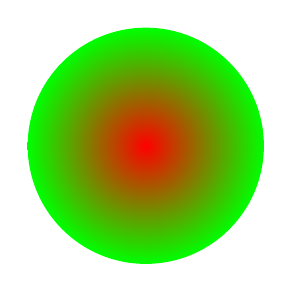
\begin{tikzpicture} % Imagen Tikz.
        			\draw[draw=none,inner color=red, outer color=green] (0,0) circle (1.5cm);
      			\end{tikzpicture}
         	\end{tikzfigure}

		}
		% Etiqueta del bloque
     	\labelblock{uso}
     	
		%%%%%%%%%%%%%%%%%%
		% Nota: con conexión al contenido
		%%%%%%%%%%%%%%%%%% 
     	\note[targetoffsetx=3cm,targetoffsety=9.5cm,innersep=.4cm,angle=-45,connection]{Esta es una nota que apunta a algo concreto del contenido}
     
		%%%%%%%%%%%%%%%%%%
		% Bloque: Ejemplo de múltiples imágenes
		%%%%%%%%%%%%%%%%%%     
%     	\block{Ejemplo de múltiples imágenes}{
%	     	{\centering    
%			\begin{tabular}{@{}rccccccc@{}} 
%			\begin{sideways}\makebox[0pt][c]{Aciertos}\end{sideways} &
%			\parbox[c]{0.11\linewidth}{\includegraphics[width=\linewidth]{archivos/l_fa_success_1.pdf}} &
%			\parbox[c]{0.11\linewidth}{\includegraphics[width=\linewidth]{archivos/l_fb_success_1.pdf}} &
%			\parbox[c]{0.11\linewidth}{\includegraphics[width=\linewidth]{archivos/l_ql_success_1.pdf}} &
%			\parbox[c]{0.11\linewidth}{\includegraphics[width=\linewidth]{archivos/l_qr_success_1.pdf}} &
%			\parbox[c]{0.11\linewidth}{\includegraphics[width=\linewidth]{archivos/l_hl_success_1.pdf}} &
%			\parbox[c]{0.11\linewidth}{\includegraphics[width=\linewidth]{archivos/l_hr_success_1.pdf}} &
%			\parbox[c]{0.11\linewidth}{\includegraphics[width=\linewidth]{archivos/l_rc_success_1.pdf}} \\
%			\midrule
%			\begin{sideways}\makebox[0pt][c]{Fallos}\end{sideways} &
%			\parbox[c]{0.11\linewidth}{\includegraphics[width=\linewidth]{archivos/l_fa_fail.pdf}} &
%			\parbox[c]{0.11\linewidth}{\includegraphics[width=\linewidth]{archivos/l_fb_fail.pdf}} &
%			\parbox[c]{0.11\linewidth}{\includegraphics[width=\linewidth]{archivos/l_ql_fail.pdf}} &
%			\parbox[c]{0.11\linewidth}{\includegraphics[width=\linewidth]{archivos/l_qr_fail.pdf}} &
%			\parbox[c]{0.11\linewidth}{\includegraphics[width=\linewidth]{archivos/l_hl_fail.pdf}} &
%			\parbox[c]{0.11\linewidth}{\includegraphics[width=\linewidth]{archivos/l_hr_fail.pdf}} &
%			\parbox[c]{0.11\linewidth}{\includegraphics[width=\linewidth]{archivos/l_rc_fail.pdf}} 
%			\end{tabular}
%			\\[1em]
%			}
%			Se puede observar que el reconocimiento facial ha sido exitoso en la mayoría de las ocasiones aunque hay algunas excepciones.
%	     }
     
%     	%%%%%%%%%%%%%%%%%%
%		% Bloque: Colores
%		%%%%%%%%%%%%%%%%%% 
%		\block{Colores}{
%		La configuración de colores puede hacerse individualmente o aprovechar algunos paquetes de colores prediseñados.
%		Las líneas que configuran los colores por separado se encuentran a continuación de la configuración de estilo. \\
%		Después de las líneas de colores individuales se encuentra el comando para elegir un paquete de colores, si se desea utilizar los colores individuales elimina el comando para paquetes de colores, ya que sobreescribirá los colores elegidos anteriormente. El comando para elegir un paquete de colores es:
%		\begin{quote}
%	         	\texttt{\bs usecolorstyle\{COLORES\}}
%	   	\end{quote}
%	   	donde ``COLORES" puede ser \texttt{TFGTFM, Default, Australia, Britain, Sweden, Spain, Russia, Denmark, Germany, Utah, Data, Qacolor, Elena}. \\
%	   	El color ``TFGTFM" utiliza en partes el mismo color que el de la titulación.
%		}

     
     	%%%%%%%%%%%%%%%%%%
		% Bloque: Estilos
		%%%%%%%%%%%%%%%%%% 
		\block{Estilos}{
	         Se han prediseñado varios conjuntos de colores y estilos de los componentes del póster (si utilizas el sistema de bloques, notas, etc).
	         Las opciones están ubicadas después de la información del trabajo y antes del comando \texttt{\bs begin\{document\}}. \\
	         Para elegir una forma de los bloques se debe realizar en la línea:
	         \begin{quote}
	         	\texttt{\bs estilobloque\{ESTILO\}}
	         \end{quote}
	         donde ``ESTILO" puede ser \texttt{TFGTFM, Default, Basic, Minimal, Envelope, Corner, Slide, TornOut, Barra}. \\
	         Para elegir una forma de los bloques internos se debe realizar en la línea:
	         \begin{quote}
	         	\texttt{\bs useinnerblockstyle\{ESTILO\}}
	         \end{quote}
	         donde ``ESTILO" puede ser \texttt{TFGTFM, Default, Table, Basic, Minimal, Envelope, Corner, Slide, TornOut}. \\
	         Para elegir una forma de las notas se debe realizar en la línea:
	         \begin{quote}
	         	\texttt{\bs usenotestyle\{ESTILO\}}
	         \end{quote}
	         donde ``ESTILO" puede ser \texttt{Default, Corner, Gradiente, Sticky}. \\
	         Para elegir un estilo de fondo se debe realizar en la línea:
	         \begin{quote}
	         	\texttt{\bs usebackgroundstyle\{ESTILO\}}
	         \end{quote}
	         donde ``ESTILO" puede ser \texttt{TFGTFM, Rayos, Gradiente, GradienteInferior, Vacio}. \\
	     }
	     \labelblock{estilos}
	     \flechacaja{estilos}{east}{}
	     
		%%%%%%%%%%%%%%%%%%
		% Nota: Ejemplo largo
		%%%%%%%%%%%%%%%%%%     
     	\note[targetoffsetx=18cm, targetoffsety=-4cm,rotate=0.5,angle=270,radius=17cm,width=.85\textwidth,innersep=.4cm]{
	         Puedes añadir notas ``ancladas" al bloque escrito anteriormente con el comando
	         \begin{quote} \texttt{\bs note[{\it opciones}]\{{\it contenido}\}}\end{quote}
	         La nota (sin opciones añadidas) se genera ligeramente a la derecha y en el centro del bloque anterior. Con las opciones se puede ajustar la posición o tamaño. \\
	         Las opciones para añadir un desfase a la posición de la nota son  \texttt{targetoffsetx, targetoffsety}, también se puede rotar con \texttt{rotate}, o especificar un ancho con \texttt{width}.  La posición de la nota respecto al bloque se establece con coordenadas polares con \texttt{ radius, angle}. Esta nota tiene las siguientes opciones \texttt{[targetoffsetx=20cm, targetoffsety=-1cm,rotate=0.5,angle=270,radius=17cm,width=.85\bs textwidth,innersep=.4cm]}
	      }

     	% Columna que ocupa el 55% del ancho de la página. Introduce el valor que desees
		\column{.45}
		% A partir de aquí todos los bloques que se escriban tendrán el ancho de la columna definida anteriormente.
		
		%%%%%%%%%%%%%%%%%%
		% Bloque: Columnas
		%%%%%%%%%%%%%%%%%% 
      	\block{Columnas}{
      		Por defecto, los bloques ocupan todo el ancho del póster (como el primer bloque de este ejemplo). Si se desea dividir el póster en columnas, se debe utilizar el entorno \texttt{columns} environment. Por ejemplo,
	         \begin{quote}
	             \texttt{\noindent \bs begin\{columns\}\\
	             \bs column\{.6\}\\
	             \bs block\{Título\}\{Contenido\}\\
	             \bs column\{.4\}\\
	             \bs block\{Título\}\{Contenido\}\\
	             \bs block\{Título\}\{Contenido\}\\
	             \bs end\{columns\}
	             }
	         \end{quote}
	         creará 2 columnas con un ancho del 60\% del póster la primera y de 40\% la segunda. La posición y espacios se ajustan automáticamente. Todo lo que se encuentre a continuación del comando \texttt{\bs column} se incluiré en el póster con el ancho de la columna. Se pueden definir tantas columnas como se deseen (también subcolumnas, ver bloque de abajo).
	     }


		%%%%%%%%%%%%%%%%%%
		% Subcolumnas
		%%%%%%%%%%%%%%%%%%  
		\begin{subcolumns}
			% Subcolumna que ocupa el 45% de la columna actual
	 		\subcolumn{.45}
	 		% Bloque
	   		\block{Subcolumnas}{Dentro de una columna definida se puede subdividir generando subcolumnas con \texttt{\bs subcolumn\{\}}, en la columna de la derecha}
			\labelblock{subcolumnas} % Etiqueta del bloque
			
			% Subcolumna que ocupa el 50% de la columna actual
	     	\subcolumn{.55}
	     	% Bloque sin título
	       	\block{}{Ejemplo de uso de subcolumnas. Se debe utilizar dentro de una columna.
	      		\begin{quote}
	                 \texttt{\bs begin\{subcolumns\}\\
	                 \bs subcolumn\{.6\}\\
	                 \bs block\{Título\}\{Contenido\}\\
	                 \bs subcolumn\{.4\}\\
	                 \bs block\{Título\}\{Contenido\}\\
	                 \bs end\{subcolumns\}
	                 }
	         	\end{quote}
	     }
         
   		\end{subcolumns}

		%%%%%%%%%%%%%%%%%%
		% FLECHAS: Ejemplo con y sin desfase de posición
		% Para más información ver la wiki en GitHub. 
		%%%%%%%%%%%%%%%%%% 
		%****************************
		\flechaA{-0.5ex} % Ajuste de la posición del texto. Negativo->abajo, Positivo->arriba	
		{white} % Color del texto
		{Flecha con desfase de posición} % Texto dentro de la flecha
		{blue} % Color de la flecha
		{[shift={(0cm,-3cm)}]uso.north east} % Inicio: Posición respecto a un bloque más desfase
		{bend left=0} % Parámetros de la recta entre los dos puntos
		{[shift={(0.5cm,0cm)}]subcolumnas.north west} % Inicio: Posición respecto a un bloque más desfase
		%***************************
		%****************************
		\flechaA{-1ex} % Ajuste de la posición del texto. Negativo->abajo, Positivo->arriba	
		{white} % Color del texto
		{Flecha sin desfase de posición} % Texto dentro de la flecha
		{red} % Color de la flecha
		{uso.south} % Inicio: Posición respecto a un bloque
		{bend right=10} % Parámetros de la recta entre los dos puntos
		{subcolumnas.west} % Inicio: Posición respecto a un bloque
		%***************************
		
		%%%%%%%%%%%%%%%%%%
		% Bloque: Tipos de bloques internos y cajas
		%%%%%%%%%%%%%%%%%% 
		\block{Tipos de bloques y cajas}{
			Diferentes tipos de bloques internos y cajas de colores:
			% Bloque interno con título
			\innerblock[]{Bloque interno}{Los bloques internos se crean dentro de los bloques con \bs\texttt{innerblock[{\it opciones}]\{{\it Título}\}\{{\it Contenido}\}} }
    		% Bloque interno sin título
    		\innerblock{}{Para obtener solo el cuadro de texto deja el título vacío. }
    		% Caja con color
    		\coloredbox[]{Puedes subrayar texto con cajas de colores utilizando  \bs\texttt{coloredbox[{\it opciones}]\{{\it Contenido\}}}}
    		% Caja con color y parámetros
    		\coloredbox[bgcolor=lightgray,framecolor=black]{Por defecto \bs\texttt{coloredbox} no tiene marco. Tanto el marco como el color se pueden definir en las opciones.}
		}
		
     \end{columns}
     
    %%%%%%%%%%%%%%%%%%
	% Pie de página. NO MODIFICAR
	%%%%%%%%%%%%%%%%%%  
   	\footer	% Genera el pie de página
   	
 \end{document}
 